
{\underline {\bf В третьей главе}} описана разработанная
модель РС, основанная на применении теории нечетких множеств
(далее будем обозначать разработанную модель НРС) и проведено теоретическое
сравнение этой модели с АКМ.\\

Будем представлять контент как нечеткое подмножество множества характеристик и
определим операции объединения и пересечения контентов:
\begin{itemize}
			\item
				$c_X(u) = \{(x | w_U(u, x )) \}, w_U(u, x) \in [0,1]$ ---
				контент пользователя, $x \in X$. При этом множество $X$ не
				обязательно является множеством $I$, как в случае с АКМ, а,
				например, в качестве характеристик может выступать контекстная
				информация.
				$w_U(u, x)$ является
				характеристической функции принадлежности;
			\item
				$c_Y(i) = \{(y | w_I(i, y )) \}, w_I(i, y) \in [0,1]$ ---
				контент объекта, $y \in Y$.
				$w_I(i, x)$ является
				характеристической функции принадлежности;
			\item
				$c_X(u) = \varnothing$, если $w_U(u, x) \equiv 0$ ---
				пустой контент пользователя;
			\item
				$c_Y(i) = \varnothing$, если $w_I(i, y) \equiv 0$ ---
				пустой контент объекта;
			\item
				$c_X(u_1) \bigcup c_X(u_2) = c_X(v): \forall x \in X$ $w_U(v, x) =
				\max(w_U(u_1, x), w_U(u_2, x))$ ---
				объединение контентов пользователей;
			\item
				$c_Y(i_1) \bigcup c_Y(i_2) = c_Y(j): \forall y \in Y$ $w_I(j, y) =
				\max(w_I(i_1, y), w_I(i_2, y))$ ---
				объединение контентов объектов;

			\item
				$c_X(u_1) \bigcap c_X(u_2) = c_X(v): \forall x \in X$ $w_U(v, x) =
				\min(w_U(u_1, x), w_U(u_2, x))$ ---
				пересечение контентов пользователей;
			\item
				$c_Y(i_1) \bigcap c_Y(i_2) = c_Y(j): \forall y \in Y$ $w_I(j, y) =
				\min(w_I(i_1, y), w_I(i_2, y))$ ---
				пересечение контентов объектов.
\end{itemize}

В качестве меры близости объектов будем использовать обобщенное расстояние Хэмминга:
    \begin{equation}
		\label{fuz:rhu}
		\rhu(u,v) =
      \begin{cases}
		  \text{Не определено, если} & c_X(u) \bigcap c_X(v) = \varnothing\\
		  \frac{1}{|X|} \cdot \sum \limits_{x \in X} |w_U(u, x) -
		  w_U(v,x)| & \text{иначе}
      \end{cases}
    \end{equation}

В качестве меры близости пользователей будем использовать обобщенное расстояние Хэмминга:
    \begin{equation}
		\label{fuz:rhi}
		\rhi(i, j) =
      \begin{cases}
         \text{Не определено, если} & c_Y(i) \bigcap
		  c_Y(j) = \varnothing \\
        \frac{1}{|Y|} \cdot \sum \limits_{y \in Y} |w_I(i, y) - w_I(j,y)| & \text{иначе}
      \end{cases}
    \end{equation}
Заданные расстояния обладают метрическими свойствами.

Определим отношение близости пользователей:
\begin{equation}
	\label{fuz:ru}
	u \ru v \Leftrightarrow \rhu(u, v) \le \varepsilon^{\prime}_p :=
	\varepsilon_p.
\end{equation}

Определим отношение близости объектов:
\begin{equation}
	\label{fuz:rt}
i \rt j \Leftrightarrow \rhi(i, j) = \varepsilon_0 := 0.
\end{equation}

Современные РС могут оперировать с контекстной информацией,
а не только информацией о предпочтениях пользователя как
в случае с АКМ.
Этой информацией может быть, к примеру,
социально-демографические данные пользователя или данные о
географическом местоположении.
Разработанная модель позволяет работать
с подобной информацией, поэтому разработанная модель является расширением
АКМ по данным о пользователе. РС производит сопоставление
информации о пользователе и объекте, за счет которого определяется
оценка близости пользователя и объекта. В случае АКМ сопоставление
определяется эвристическими утверждениями.
При работе с более широкой и
неоднозначной информацией о пользователе и при ее сопоставлении с данными об
объектах могут применяться знания эксперта, алгоритмические подходы такие, к примеру,
как машинное обучение и т.д.

В разработанной модели сопоставление информации и пользователе и объекте
определяется заданием
нечеткого отображения $\dc: X \times Y \rightarrow [0,1]$, именуемым оценкой
близости характеристик.

Функция сходства $\dc$ может быть задана в табличной или
аналитической форме алгоритмически или экспертом.

Зададим функцию принадлежности при нечетком отображении $\Psi$ следующим образом:
\begin{equation}
	\label{make-rho1}
		\nu_{\Psi}(y) = \underset{x \in X} {\mathrm{\max}} \min\{
			\delta_c(x,y); w_U(u, x) \}
\end{equation}

С помощью функции $\dc$ можно определить нечеткое отображение $\Psi: X \rightarrow Y$ контента
пользователя на множество контентов объектов.
Для этого
зададим характеристическую функцию принадлежности $\nu_{\Psi}$ характеристики
$y$ нечеткому подмножеству универсального множества $Y$ при отображении $\Psi$ следующей формулой:
\begin{equation}
	\nu_{\Psi}(y) = \underset{x \in X} {\mathrm{\max}} \min\{ \rho(x,y); \mu(x) \}
\end{equation}

Определим функцию отображения контентов пользователей:
\begin{equation}
	\Psi(c_X(u)) = \{ (y | \nu_{\Psi}(y)) \}, y \in Y
\end{equation}

При наличии способа отображения контента пользователя, зададим расстояние
между пользователем $u$ и объектом $i$, значение которого будет выступать в
роли значения прогнозной функции:
	\begin{equation}
		\label{my-rh}
		\rh(u,i) := \rhi(\overline{i}, i)\text{, где }
		c_Y(\overline{i}) := \Psi(c_X(u))
	\end{equation}

\begin{equation}
	\begin{aligned}
	\label{my-pi}
		\text{Нечеткое правило $\Pi_f$ НРС }\\
	\text{заключается в задании оценки сходства } \delta_c\\
	\text{и в дальнейшем расчете прогнозной функции }\rh
	\end{aligned}
\end{equation}

Определим НРС следующим образом:
	\begin{multline}
		(c_X(u) = \{(x | w_U(u, x )) \},\\
		 c_Y(i) = \{(y | w_I(i, y )) \},\\
		\Pi \in \{\Pi_{O}, \Pi_{C}, \Pi_f\}
	\end{multline}
НРС включает правила вывода АКМ,
и поэтому является ее расширением.

{\bf Решения задач в нечеткой модели}.
Определим решения в НРС при использовании $\Pi_f$. Задача $topN$ может быть решена
с помощью линейного поиска объектов, близких к активному пользователю (Рис. 3).
\begin{figure}[H]
	\caption{Алгоритм решения задачи $topN$}
	\begin{center}
		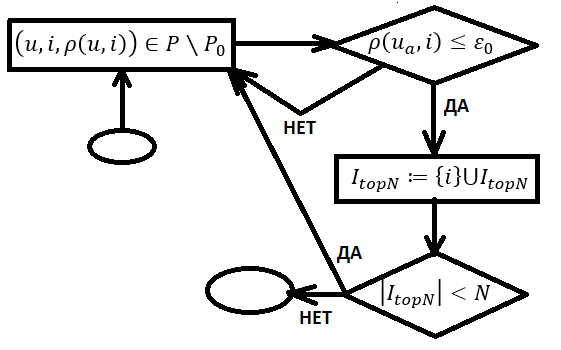
\includegraphics[width=4in,height=2in]{pics/topn-fuz-no-box.png}
	\end{center}
\end{figure}

Задача прогнозирования заключается в вычислении расстояния $\rh(u_a, i_{\bot})$ между
активным пользователем и прогнозируемым объектом.
\begin{figure}[H]
	\caption{Алгоритм решения задачи $topN$}
	\begin{center}
		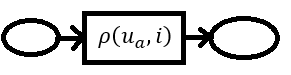
\includegraphics[width=3in,height=1in]{pics/prdn-fuz.png}
	\end{center}
\end{figure}

При решении задачи $topN$ максимальное число вычислений $\rh$ равно $n$,
поэтому асимптотическая сложность алгоритма решения равна $O(n)$. Для решения
задачи $pred$ единожды проводится вычисление расстояния,
поэтому асимптотическая сложность алгоритма решения равна $O(1)$.

Проведем сравнение качества НРС и АКМ.

{\bf Сравнение моделей по критерию вычислительной сложности}.
В таблице <<Сравнение асимптотических сложностей>> (\ref{tbl:complex})
приведены асимптотически сложности алгоритмов решений задач в АКМ и НРС.

\begin{table}[h]
	\caption{Сравнение асимптотических сложностей}
	\label{tbl:complex}
  \begin{center}
  \begin{tabular}{|c|c|c|c|}
	\hline
	Модель & Задача & Сложность  \\ \hline
	АКМ & $topN$ & $O(n^2)$  \\ \hline
	АКМ & Прогнозирование & $O(m)$ \\ \hline
	НРС & $topN$ & $O(n)$ \\ \hline
	НРС & Прогнозирование & $O(1)$ \\ \hline
  \end{tabular}
\end{center}
\end{table}
Асимптотические сложности решений задач в НРС
при использовании правила $\Pi_f$ на порядок меньше сложностей
КМ.

{\bf Сравнение моделей по критерию качества решения}.
Рассмотрим качество решений задач по критерию качества
в НРС при использовании $\Pi_O$ и $\Pi_C$.

При решении задачи $pred$ в НРС при применении $\Pi_C$
будем строить кластер соседей следующим образом:
$\mathcal{N}_U = \{ u : \rhu(u_a, u) \le \frac{1}{2} \cdot \varepsilon_p \wedge
(u, i_{\bot}, \rho(u, i_{\bot})) \in P_0)$ \}.
При таком построении кластера выполняется
достаточное условие качественного решения,
что обусловлено
метрическими свойствами используемой в НРС
меры близости $\rhu$ (\ref{fuz:rhu}).

%Покажем, что выполняется достаточное условие. Напомним, что оно
%заключается в выполнении свойства транзитивности отношения близости $\ru$ на
%кластере соседей.
%$\forall u, v \in \mathcal{N}_U$ верно, что
%$(u_a \ru u) \wedge (u_a \ru v)$. Так как функция $\rhu$ обладает
%метрическими свойствами, то $\rhu(u, v) \le \rhu(u_a, u) + \rhu(u_a, v)$.
%По дополнительному условия
%$\rhu(u_a, u) \le \frac{1}{2} \cdot \varepsilon_0$,
%$\rhu(u_a, v) \le \frac{1}{2} \cdot \varepsilon_0$,
%поэтому $\rhu(u, v) \le \varepsilon_p \Rightarrow u \ru v$.

При решении задачи $topN$ в НРС при применении $\Pi_O$
выполняется достаточное условие качественного решения,
что обусловлено заданием отношения $\rt$ (\ref{fuz:rt})
в НРС и метрическими свойствами используемой в
НРС меры близости $\rhi$ (\ref{fuz:rhi}).

Так как в НРС при использовании $\Pi_C$ и $\Pi_O$
выполняются достаточные условия качественных решений, то
разработанная модель является качественной модификацией АКМ.

Эффективность НРС по критерию качества при применении правила
вывода $\Pi_f$ так же, как и в АКМ ограничена
дополнительным условием.
В обеих моделях выполнение условий
зависит от разработчика: для АКМ это выбор функции $\rhi, \rhu$ и порогового
значения $\varepsilon_i, \varepsilon_u$, для НРС --- это
определение $\delta_c$.
Однако при работе с АКМ
разработчик обладает меньшей свободой действий, чем при работе с
НРС, так как он может варьировать только функцию, которая будет
использоваться в качестве меры близости, и ее пороговое значение.
При работе с НРС разработчик может варьировать
алгоритмы, эвристики, наборы данных, знания
экспертов и т.п., чтобы задать $\delta_c$ и зависящее от этой функции $\Pi_f$.

{\bf Вывод}: разработана математическая модель РС, которая теоретически
более качественна, чем АКМ, и является ее расширением.
